% Chapter on Asynchronous Distributed Adaptive Gradient
%
% Developed for my Master Thesis at Maastricht University.
% Based on Eugenio Senes's template at the University of Torino.
%
% By Joeri Hermans (joeri@joerihermans.com)
%
% Released under an MIT license. Share, modify and enjoy, but quote the author!

\chapter{Accumulated Gradient Normalization}
\label{chapter:accumulated_gradient_normalization}

This chapter addresses the first contribution of this thesis, which is \emph{accumulated gradient normalization}, or \textsc{agn} in short. We start by laying out the concept and intuition behind accumulated gradient normalization, and show why \textsc{agn} provides the central variable with more efficient updates. Finally, to show our claims, we provide several experiments where we compare \textsc{agn} with different distributed optimizers such as \textsc{donwpour}~\cite{dean2012large}, \textsc{aeasgd}~\cite{zhang2015deep}, and \textsc{dynsgd}~\cite{jiang2017heterogeneity}.

\section{Concept and intuition}
\label{sec:agn_concept}

The main issue with \textsc{downpour}~\cite{dean2012large} is the requirement of constant communication with the parameter server after every gradient computation. Furthermore, as the number of parallel workers increases, \textsc{downpour} fails to converge due to the amount of \emph{implicit momentum}~\cite{implicitmomentum}, as shown in Figure~\ref{fig:downpour_convergence}. To reduce the amount of communication with the parameter server, one could take ideas from \textsc{easgd}~\cite{zhang2015deep}, and perform several iterations of local exploration before committing the gradients to the parameter server. However, in the case of algorithms like \textsc{downpour}, that is, where gradients are committed to the parameter server in an asynchronous fashion, more local exploration results in proportionally larger gradients, and as a result, complicate the staleness and the implicit momentum problem even further as adressed in Chapter~\ref{chapter:asynchronous_distributed_adaptive_gradients}. To intuitively show why this is an issue, let us consider Figure~\ref{fig:downpour_accumulation_issue}. In a regular \textsc{downpour} setting, first-order gradients such as in Subfigure (a) are committed to the parameter server. However, when an algorithm allows for a certain amount of local exploration, such as Algorithm~\ref{algo:downpour_worker_zealous}, the gradient that is committed to the parameter server is an \emph{accumulated gradient} as shown in Subfigure (b).

\begin{figure}[H]
  \centering
  \begin{subfigure}{.49\textwidth}
    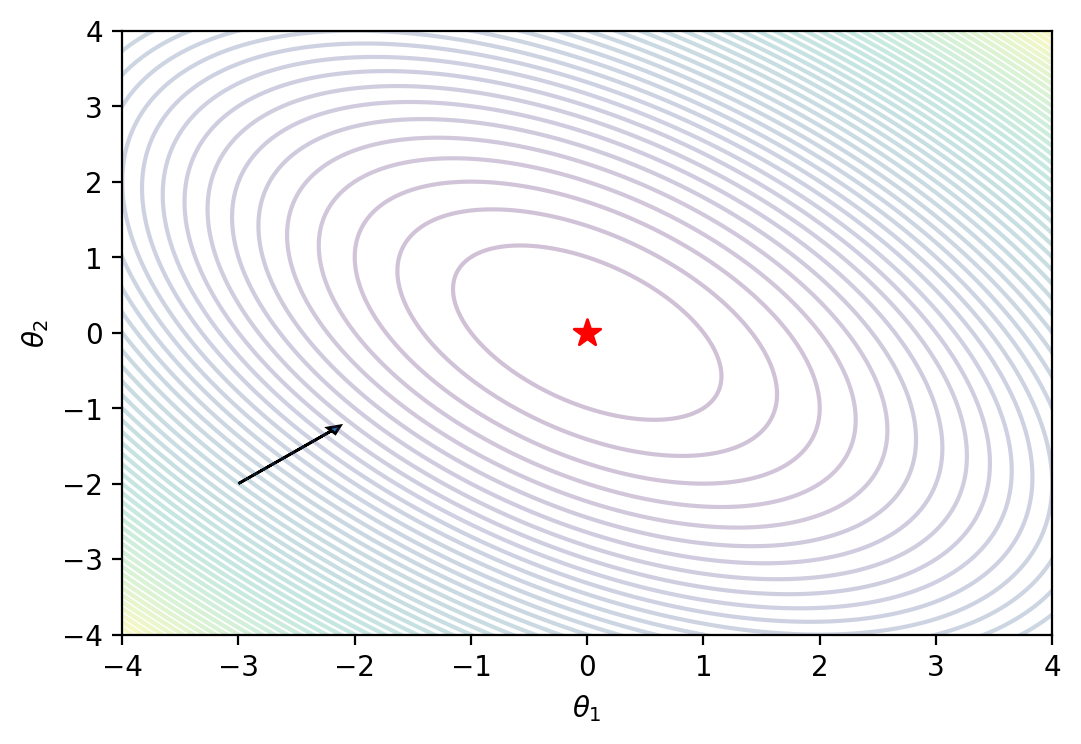
\includegraphics[width=\linewidth]{resources/images/agn_no_accumulated}
    \caption{No Gradient Accumulation}
  \end{subfigure}
    \begin{subfigure}{.49\textwidth}
    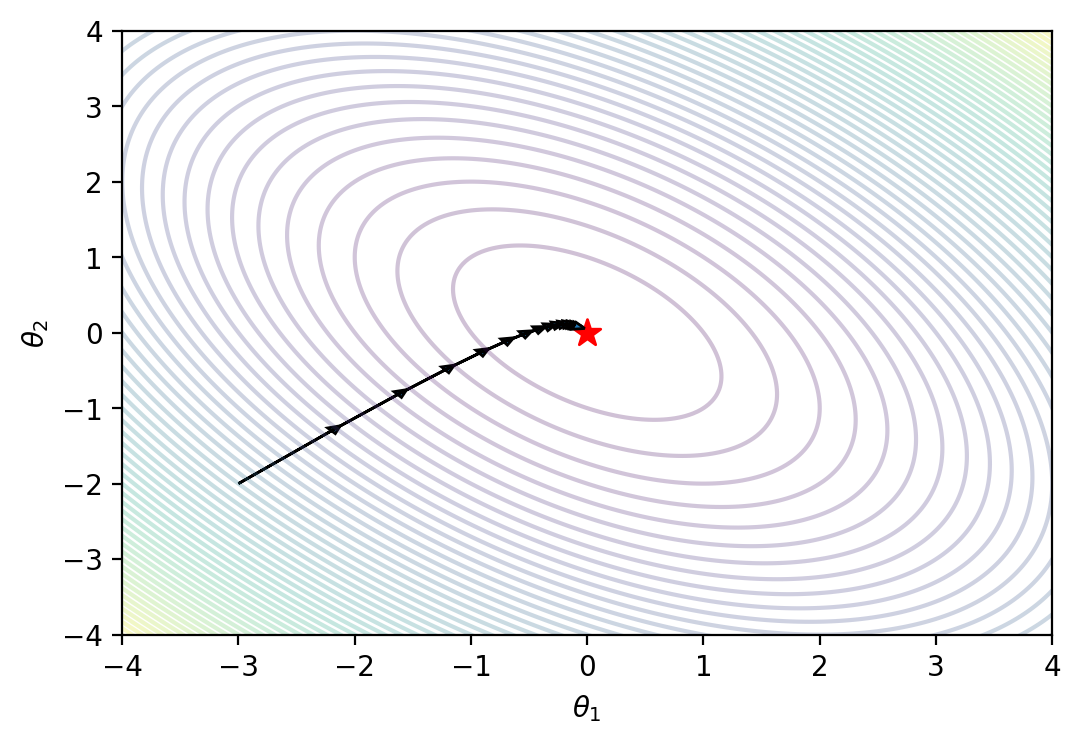
\includegraphics[width=\linewidth]{resources/images/agn_accumulated}
    \caption{Gradient Accumulation}
  \end{subfigure}
  \caption{This figure shows the difference between regular first-order gradients (a), and accumulated gradients (b). We observe that \emph{accumulated gradients are proportionally larger to the number of exploration steps}. However, they do provide a better direction compared to first-order gradients.}
  \label{fig:downpour_accumulation_issue}
\end{figure}

Now, imagine two asynchronous environments, in the first no gradient accumulation is performed, and in the last gradient accumulation takes place. In the environment where no gradient accumulation is performed, as in regular \textsc{downpour}, first-order gradients are committed to the parameter server. However, as we have seen in Chapter~\ref{chapter:distributed_deep_learning}, and in particular Figure~\ref{fig:downpour_convergence}, we saw that \textsc{downpour} diverges when the number of asynchronous workers is too high due to the amount of implicit momentum~\cite{implicitmomentum}. As a result, careful tuning is required when no adaptive methods are applied. Nevertheless, given the fact that \textsc{downpour} converges with $n = 10$ workers in Figure~\ref{fig:downpour_convergence} and our knowledge about gradient accumulation, i.e., \emph{accumulated gradients that are committed are proportional to the number of exploration steps for every worker, and provide better directions to a minimum}, we would expect that for some amount of local exploration while using the same hyperparameterization (with the exception of local exploration steps $\lambda$) \textsc{downpour} would diverge again due to the magnitude of the accumulated gradients. This behaviour is illustrated in Figure~\ref{fig:downpour_accumulated_divergence}.\\

\begin{figure}[H]
  \centering
  \begin{subfigure}{.49\textwidth}
    \centering
    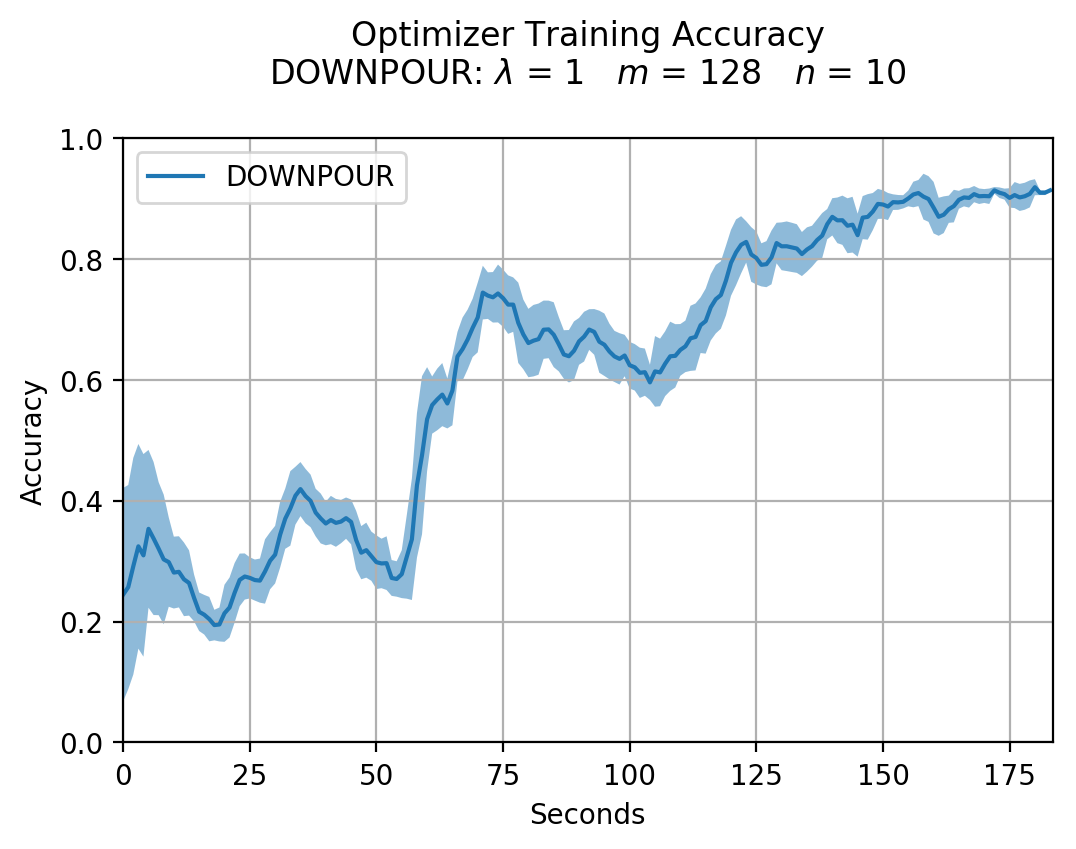
\includegraphics[width=\linewidth]{resources/images/downpour_10}
    \caption{$\lambda = 1$}
  \end{subfigure}
  \begin{subfigure}{.49\textwidth}
    \centering
    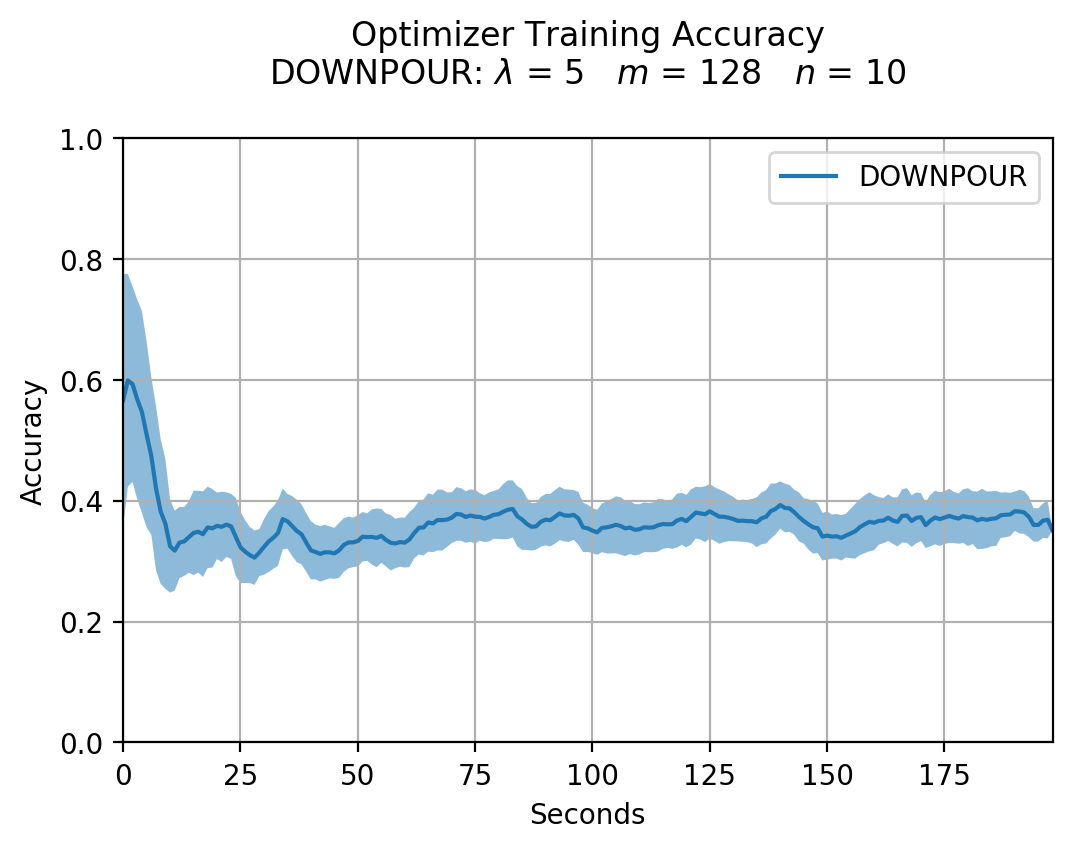
\includegraphics[width=\linewidth]{resources/images/downpour_accumulated_5}
    \caption{$\lambda = 5$}
  \end{subfigure}
   \begin{subfigure}{.49\textwidth}
    \centering
    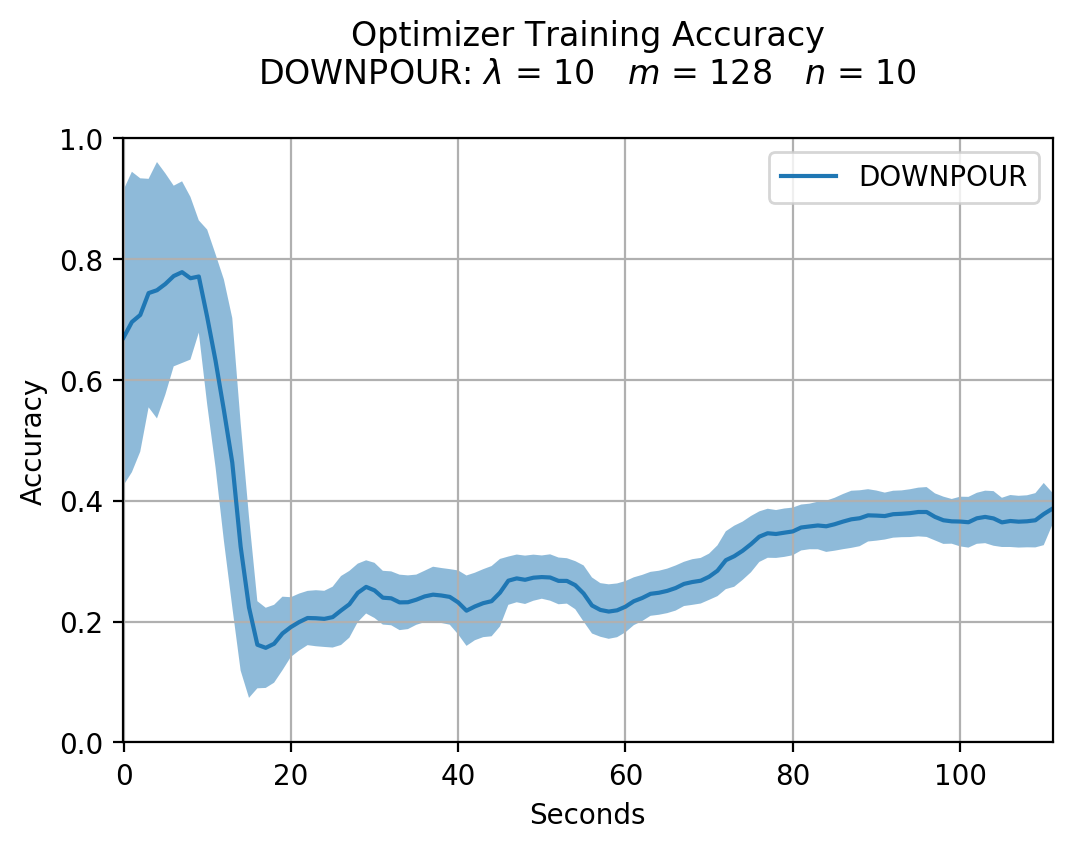
\includegraphics[width=\linewidth]{resources/images/downpour_accumulated_10}
    \caption{$\lambda = 10$}
  \end{subfigure}
  \begin{subfigure}{.49\textwidth}
    \centering
    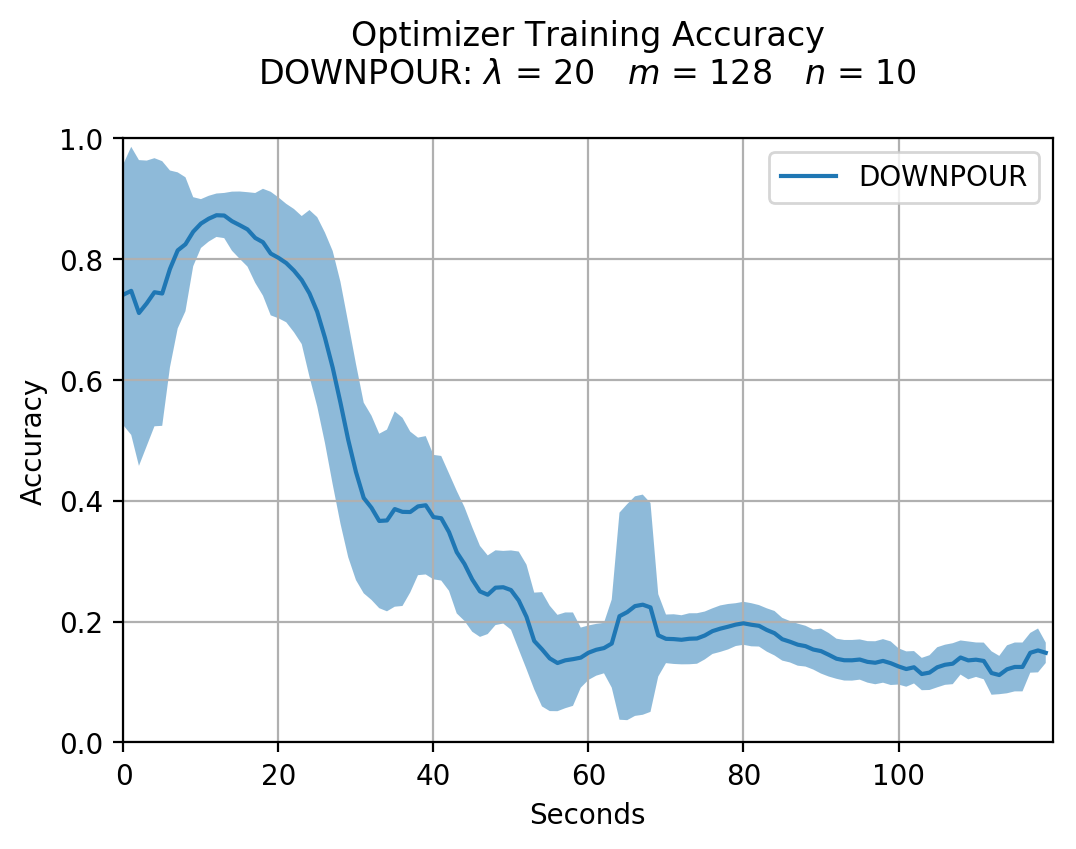
\includegraphics[width=\linewidth]{resources/images/downpour_accumulated_20}
    \caption{$\lambda = 20$}
  \end{subfigure}
  \caption{Illustration of divergence due to gradient accumulation in \textsc{downpour}. In Figure~\ref{fig:downpour_convergence}, we say that for $n = 10$ \textsc{downpour} converged to a good solution. In order to reduce the training time, we decrease the communication frequency (increasing $\lambda$). However, due to the larger gradients that are committed to the parameter server, which increases the amount of implicit momentum, the central variable is not able to converge as before.}
  \label{fig:downpour_accumulated_divergence}
\end{figure}

To reduce the magnitude of the accumulated gradients, and thereby reducing the amount of implicit momentum, while at the same time preserving the better direction that has been provided due to the amount of local exploration, we propose to normalize (average) the accumulated gradient with the amount of local steps that have been performed by the workers ($\lambda$), shown in Equation~\ref{eq:accumulated_gradient_normalization}\footnote{Note if $\lambda = 1$, \textsc{agn} is in essence equivalent to \textsc{downpour}.}. We call this technique of normalizing the accumulated gradient \emph{Accumulated Gradient Normalization} or \textsc{agn}. An initial critique of this technique would be that by normalizing the accumulated gradient, \textsc{agn} would in effect be undoing the work that has been done by a single worker. This seems at first a valid criticism, however, one needs to take into account that \textsc{agn} is actually using the worker exploration steps to compute a better gradient based on first-order gradients.

\begin{equation}
  \label{eq:accumulated_gradient_normalization}
  \Delta\theta = -\frac{\sum_{i = 0}^\lambda \eta_t \frac{1}{m}\sum_{j = 0}^{m - 1} \nabla_\theta \mathcal{L}(\theta_i;\textbf{x}_{ij};\textbf{y}_{ij})}{\lambda}
\end{equation}

Since \textsc{agn} is using local steps to compute a better gradient compared to first order gradients, it can also be used under communication constraints like \textsc{easgd} since less communication with the parameter server is required. In Figure~\ref{fig:agn_example}, we show how a \emph{Normalized Accumulated Gradient} is obtained and applied to the central variable using Equation~\ref{eq:accumulated_gradient_normalization} as described using Algorithm~\ref{algo:agn}.

\begin{figure}[H]
  \centering
  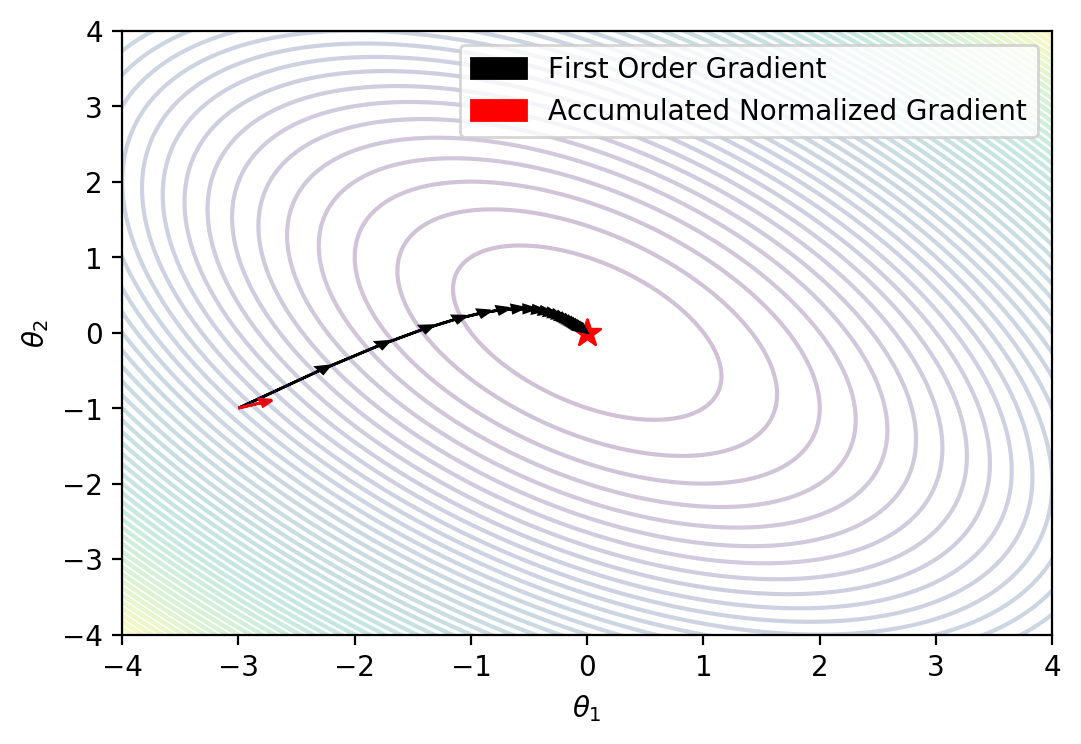
\includegraphics[width=.45\textwidth]{resources/images/agn_example}
  \caption{After pulling the most recent parameterization of the central variable from the parameter server, the worker starts accumulating $\lambda$ first order gradients, and applies those gradients locally to explore the surrounding error space. Finally, after $\lambda$ exploration steps have been performed, the accumulated is normalized w.r.t. $\lambda$ and send to the parameter server.}
  \label{fig:agn_example}
\end{figure}

\begin{algorithm}[H]
  \caption{Worker procedure of \textsc{agn}.}
  \label{algo:agn}
  \begin{algorithmic}[1]
    \Procedure{AGNWorker}{$k$}
    \State $\theta^k_0 \gets \tilde{\theta} \gets \Call{Pull}$
    \State $t \gets 0$
    \While{$\textbf{not}$ converged}
    \State $i \gets 0$
    \State $a \gets 0$
    \While{$i < \lambda$}
    \State $\textbf{x},~\textbf{y} \gets \Call{FetchNextMiniBatch()}{}$
    \State $g \gets -\eta_t \odot \nabla_\theta \mathcal{L}(\theta^k_t;\textbf{x};\textbf{y})$
    \State $a \gets a + g$
    \State $\theta^k_{t + 1} = \theta^k_t + g$
    \State $i \gets i + 1$
    \State $t \gets t + 1$
    \EndWhile
    \State $a \gets \frac{a}{\lambda}$ \Comment{Accumulated Gradient Normalization step.}
    \State $\Call{Commit}{g}$
    \State $\theta^k_{t + 1} \gets \Call{Pull}$
    \EndWhile
    \EndProcedure
  \end{algorithmic}
\end{algorithm}

\begin{equation}
  \lim_{\lambda \to \infty} -\frac{\sum_{i = 0}^\lambda \eta_t \frac{1}{m}\sum_{j = 0}^{m - 1} \nabla_\theta \mathcal{L}(\theta_i;\textbf{x}_{ij};\textbf{y}_{ij})}{\lambda}
\end{equation}
